It is unlikely to have a model perform as one expects the first time. There are
therefore a few techniques for optimizing the performance. It should be noted
that much of the discussion here and in Section \ref{sec:validation} focuses on
the diagnostics aspect rather than the validation aspect of these techniques.
In practice, these are used for both purposes, but in this work the formal
comparison of model performance will be used, introduced and demonstrated in
Sections \ref{sec:invcompare} and \ref{sec:algcompare}, respectively. 

However, the increase in performance from over-optimization could be linked to
the training set performance and might not generalize outside of the specific
type of input data used.  A workaround for this scenario is to obtain more data
for the set or to obtain a completely different data set altogether. 

\subsubsection{Training Set Size}

The first diagnostic plot for optimizing the model performance is called a
\textit{learning curve}, which provides information about the bias-variance
tradeoff with respect to the data set size. More specifically, learning curves
compare the training and cross-validation errors to the size of the training
set (i.e., number of instances in the training set). This is done by randomly
selecting a percentage of the the training set, inputting that into a
statistical learner, and tabulating the error of the learned model. 

Typically, a learning curve will look somewhat like one of the three examples
in Figure \ref{fig:learning}.  A learning curve tests the model for high bias
or high variance, which can correspond to an undefit or overfit model,
respectively. 

\begin{figure}[!hp]
  \centering
  \begin{subfigure}[h]{0.65\linewidth}
    \centering
    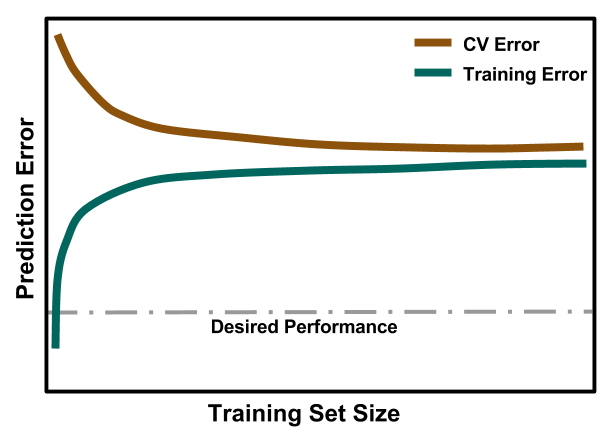
\includegraphics[width=\linewidth]{./chapters/litrev/LearningCurve-bias.png}
    \caption{High bias}
    \label{fig:bias}
  \end{subfigure}
  \begin{subfigure}[h]{0.65\linewidth}
    \centering
    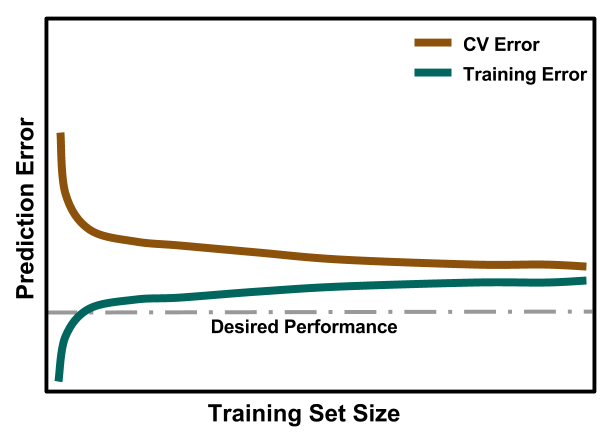
\includegraphics[width=\linewidth]{./chapters/litrev/LearningCurve-ideal.png}
    \caption{Ideal}
    \label{fig:ideal}
  \end{subfigure}
  \begin{subfigure}[h]{0.65\linewidth}
    \centering
    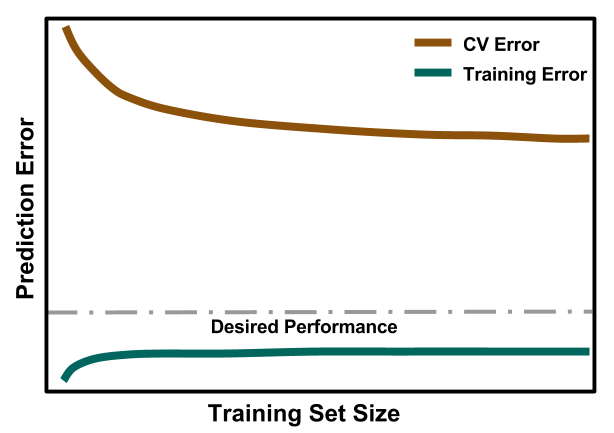
\includegraphics[width=\linewidth]{./chapters/litrev/LearningCurve-variance.png}
    \caption{High variance}
    \label{fig:variance}
  \end{subfigure}
  \caption{Learning curves for three training scenarios}
  \label{fig:learning}
\end{figure}
\todo{add reference}

Figure \ref{fig:bias} suggests underfitting because the model is missing
important features in the data. It is characterized by a small gap between the
curves but high overall errors. The cross-validation error remains consistently
high and the training error increases drastically with increasing data, since
it is not generalizing well. 

Figure \ref{fig:variance} suggests overfitting because the model has too much
sensitivity to variations in the data. It is characterized by a very large gap
between the curves. It has an extremely low training error, as it has taken
into account every detail of the training set, but a high cross-validation
error because it cannot generalize beyond the testing set. 

Figure \ref{fig:ideal} is an example of a more ideal model fit. It is
characterized by a small gap between the two errors, and they are at a
reasonable level with respect to the desired performance.  The training error
should increase with respect to the training set size due to a larger amount of
bias (preventing overfitting). But the cross-validation error should decrease
quickly with respect to the training set size due to being close to the minimum
of the bias-variance tradeoff. 

\subsubsection{Model Complexity}

After ensuring the appropriate training set size is selected, the models must
be further optimized using \textit{validation curves}.  These provide
information on the bias-variance tradeoff with respect to model complexity. Two
main factors affecting model complexity can cause the model to be under- or
overfit to the data: number of features in the data set and algorithm
parameters that vary the regularization.

%%%%%%%%%%%%%%%%%%%%%%%%%%%%%%%%%%%%%%%%%%%%%%%%%%%%%%%%%%%%
%%%%%%%%%%%%%%%%%%%%%%%%%%%%%%%%%%%%%%%%%%%%%%%%%%%%%%%%%%%%
\textit{Regularization} is a component of many machine learning aglorithms a
%%%%%%%%%%%%%%%%%%%%%%%%%%%%%%%%%%%%%%%%%%%%%%%%%%%%%%%%%%%%
%%%%%%%%%%%%%%%%%%%%%%%%%%%%%%%%%%%%%%%%%%%%%%%%%%%%%%%%%%%%

\begin{figure}[!htb]
  \centering
  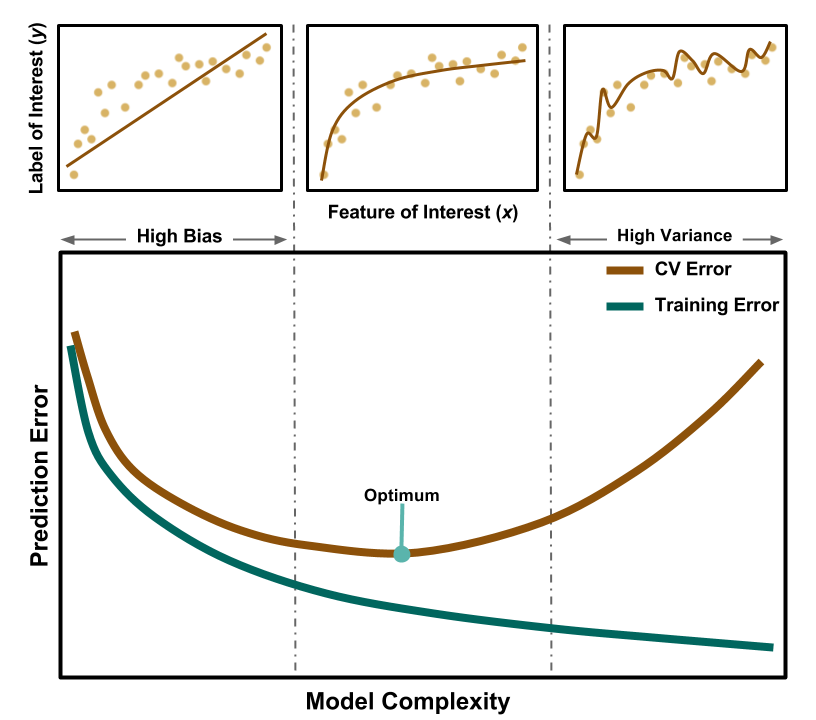
\includegraphics[width=1.05\linewidth]{./chapters/litrev/ValidationCurve.png}
  \caption{Validation curve showing examples of different fittings}
  \label{fig:validation}
\end{figure}

describe figure

In practice, plotting learning and validation curves can be iterative. But as
previously mentioned, too many optimizations will result in a poorly performing
model when exposed to data outside of the training set.

%%%%%%%%%%%%%%%%%%%%%%%%%%%%%%%%%%%%%%%%%%%%%%%%%%%%%%%%%%%%
%%%%%%%%%%%%%%%%%%%%%%%%%%%%%%%%%%%%%%%%%%%%%%%%%%%%%%%%%%%%
\subsubsection{Comparison of Methods}
\label{sec:invcompare}
%%%%%%%%%%%%%%%%%%%%%%%%%%%%%%%%%%%%%%%%%%%%%%%%%%%%%%%%%%%%
%%%%%%%%%%%%%%%%%%%%%%%%%%%%%%%%%%%%%%%%%%%%%%%%%%%%%%%%%%%%

Inverse stuff.

Priors given by set of forward problems (input data space - ORIGEN sims)

Likelihood given by model space, e.g.: 

Model params as determined from ML alg

(related) MLE from bayesian inference

Direct inversion of matrix A

Expert-elicited params (i.e. initial guesses for INDEPTH? Or optimized ones?)

Marginal likelihood only needed for absolute measures - doesn’t affect relative probabilities

